\documentclass[12pt]{article}
\usepackage{amsmath, amssymb}
\usepackage{geometry}
\usepackage{listings}
\usepackage{xcolor}
\usepackage{parskip}
\usepackage{longtable}
\usepackage{booktabs}
\usepackage{tikz}
\usepackage{pdflscape}
\usepackage{caption}
\usetikzlibrary{shapes.geometric, arrows.meta, positioning, calc}

\geometry{margin=1in}

% SQL listing style
\lstdefinestyle{sql}{
    language=SQL,
    basicstyle=\ttfamily\small,
    keywordstyle=\color{blue}\bfseries,
    commentstyle=\color{gray},
    stringstyle=\color{red},
    showstringspaces=false,
    frame=single,
    breaklines=true,
    numbers=none,
    morekeywords={VIEW, REPLACE, EXISTS, COALESCE, DATEDIFF, DATE_ADD, CURDATE, CONCAT, INTERVAL},
}

% E-R diagram styles
\tikzset{
    entity/.style={rectangle, draw, thick, minimum width=2cm, minimum height=0.8cm, fill=blue!8},
    relationship/.style={diamond, draw, thick, aspect=2, fill=yellow!15, minimum width=1.2cm, inner sep=1pt},
    attribute/.style={ellipse, draw, thin, minimum width=0.6cm, font=\footnotesize, inner sep=2pt},
    total/.style={double, thick},
    partial/.style={thick},
    tablebox/.style={rectangle, draw, thick, fill=blue!5, minimum width=2.8cm, minimum height=0.7cm, font=\small\ttfamily},
}

\title{CPSC 3660 --- Course Project Report\\[0.3cm]
\Large Lethbridge JonesAuto\\Database Management System}
\author{[Student Name] --- [Student ID]}
\date{April 8, 2026}

\begin{document}
\maketitle
\thispagestyle{empty}
\vfill
\begin{center}
CPSC 3660 --- Introduction to Database Systems\\
Winter 2026\\[0.3cm]
Professor: [Professor Name]
\end{center}
\newpage

%==============================================================
\section{Introduction}

JonesAuto is a used car dealership based in Lethbridge. They buy cars at auctions, fix them up, and resell them to customers. A lot of their sales are financed, so they have to keep track of monthly payments on top of everything else. Right now they do all of this on paper, which honestly gets pretty messy once you are dealing with dozens of cars and customers at the same time.

I built a database system to replace that whole paper-based workflow. It covers the full lifecycle of a car: buying it at auction, recording what repairs it needs, selling it to a customer, setting up warranty coverage, and tracking monthly payments. The prof talked in the first couple weeks about why a DBMS beats flat files; things like data redundancy, consistency problems, and not being able to query anything easily. This project is pretty much that idea applied to a real business. The system runs on PHP and MySQL, using WAMP as the local development server.

The system has three main parts: input forms for entering data, output reports for pulling summaries, and a queries page for answering specific business questions. There are 6 forms, 6 reports, and 12 queries total. Seven of those queries use advanced SQL features like JOINs, subqueries, and GROUP BY with HAVING. I tried to cover a good range of what we learned in class throughout the semester.

%==============================================================
\section{Stage 1: Overall Design}

\subsection{System Goals}

The main goal was to replace JonesAuto's paper records with a proper database system. The system needs to track the full car lifecycle from purchase at auction all the way through to customer payments. It also needs to give employees quick access to customer info, vehicle history, and financial summaries without digging through filing cabinets.

\subsection{Input Forms}

\begin{tabular}{ll}
\toprule
\textbf{Form} & \textbf{Purpose} \\
\midrule
Purchase Form & Records a car bought at auction with vehicle details, price, buyer, repairs \\
Sale Form & Records a car sale with financing, customer info, employment history \\
Warranty Form & Adds warranty coverage to an existing sale \\
Payment Form & Records monthly payments, detects late payments, updates credit stats \\
Customer Form & Adds new customers and shows existing customer records \\
Employee Form & Adds new employees (buyers/salespeople) and shows existing records \\
\bottomrule
\end{tabular}

\subsection{Output Reports}

\begin{tabular}{ll}
\toprule
\textbf{Report} & \textbf{Purpose} \\
\midrule
Current Inventory & Shows available cars on the lot, filterable by make, with repair cost totals \\
Sales Summary & Shows completed sales with profit calculation, filterable by date range \\
Payment History & Shows payment records for a selected customer, highlights late payments \\
Repair Costs & Compares estimated vs actual repair costs, highlights overruns \\
Active Warranties & Lists warranty coverage with color-coded expiry urgency \\
Late Payments & Shows customers with late payments, sorted worst-first \\
\bottomrule
\end{tabular}

\subsection{System Users}

There are three types of users: buyer employees who go to auctions and fill out purchase forms, salesperson employees who handle sales and warranties and payments, and office staff who run reports and queries. The system does not have a login since it is a small dealership and everyone pretty much shares the same machine.

\subsection{Initial Design Assumptions}

\begin{itemize}
  \item Cars are only acquired through auctions (though there is an \texttt{is\_auction} flag for flexibility)
  \item Each car has exactly one purchase record and at most one sale
  \item Customers can buy multiple cars over time
  \item Warranties are tied to a specific sale, not directly to a customer
  \item The dealership is in Lethbridge, Alberta (all sample data uses Alberta locations)
  \item Payments are monthly, and ``late'' means \texttt{paid\_date} is after \texttt{due\_date}
\end{itemize}

I made these assumptions based on the business description in the project spec. Some of them I had to decide on my own since the spec did not cover every edge case.

%==============================================================
\section{Stage 2: E-R Diagram and Database Schema}

The prof covered E-R diagrams in Weeks 10 and 11 using Chen notation, where you draw rectangles for entities, diamonds for relationships, and ovals for attributes. I designed the E-R diagram before writing any SQL, since mapping from an E-R model to relational tables is way more structured than jumping straight to CREATE TABLE statements. The prof's 4-step database design process was helpful here: understand the data needs, build a conceptual design with E-R, specify the operations, then do the logical and physical design.

The full E-R diagram for JonesAuto is on the following page (Figure~\ref{fig:er-diagram}). The diagram shows all 10 entity sets, the 11 relationships between them, primary keys (underlined), and cardinality labels. Double lines indicate total participation (the entity must participate in the relationship), and single lines indicate partial participation.

%--------------------------------------------------------------
% E-R DIAGRAM (landscape page)
%--------------------------------------------------------------
\begin{landscape}
\begin{figure}[p]
\centering
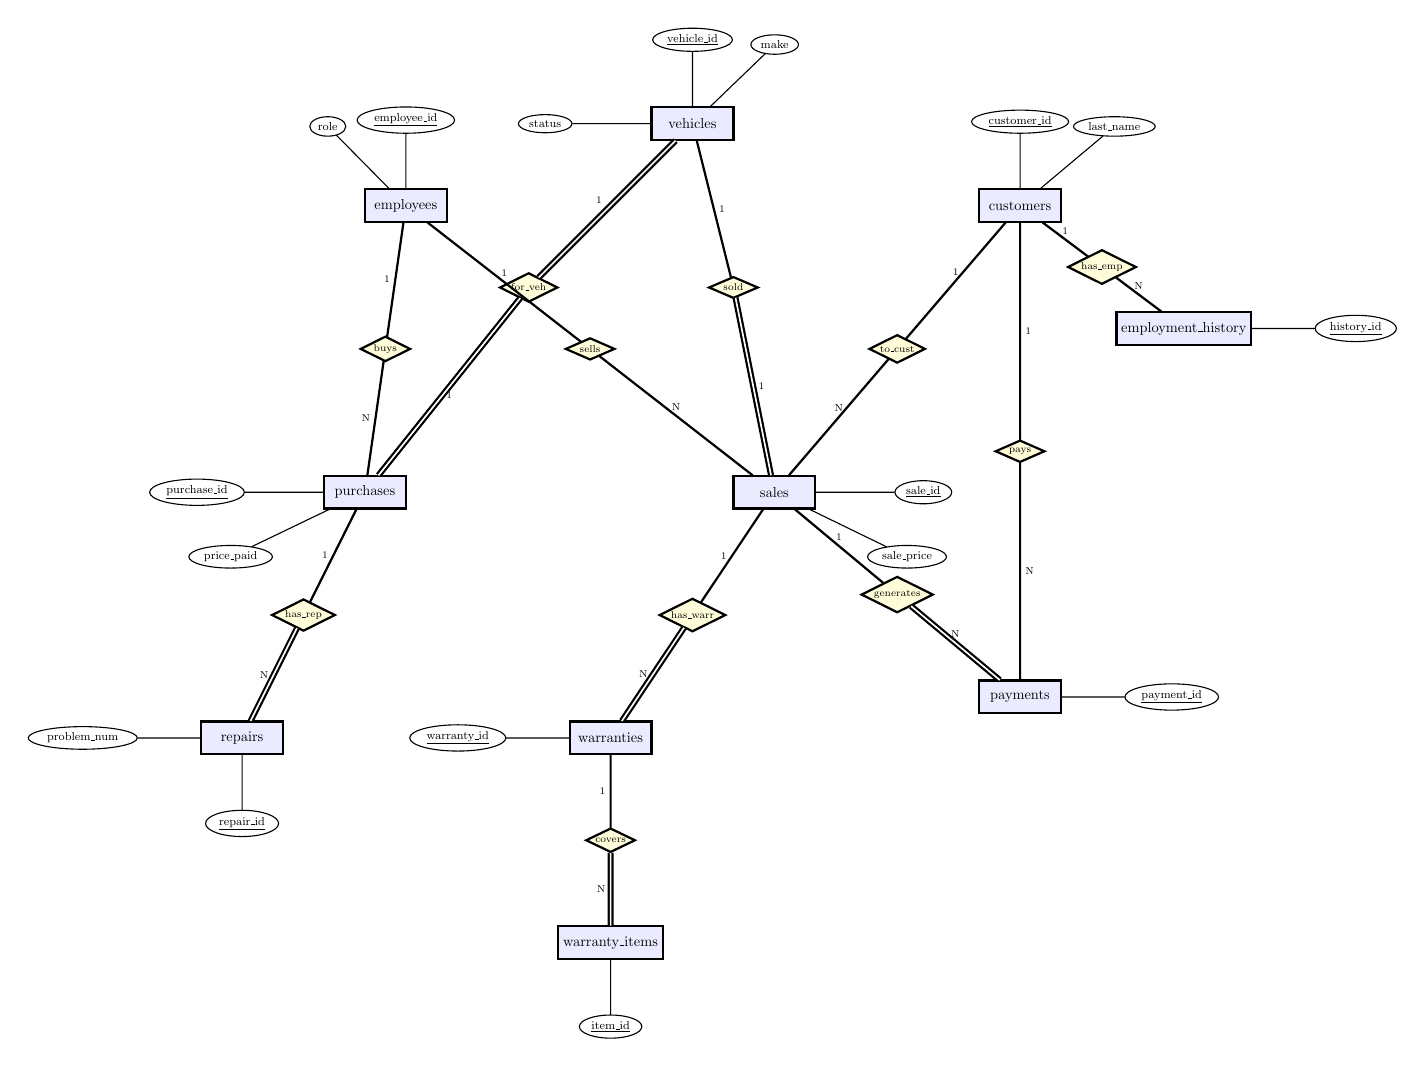
\begin{tikzpicture}[node distance=1cm, scale=0.52, every node/.style={scale=0.52}]

% === ENTITIES ===
\node[entity] (emp) at (3, 0) {employees};
\node[entity] (veh) at (10, 2) {vehicles};
\node[entity] (cust) at (18, 0) {customers};
\node[entity] (pur) at (2, -7) {purchases};
\node[entity] (sal) at (12, -7) {sales};
\node[entity] (eh) at (22, -3) {employment\_history};
\node[entity] (rep) at (-1, -13) {repairs};
\node[entity] (war) at (8, -13) {warranties};
\node[entity] (pay) at (18, -12) {payments};
\node[entity] (wi) at (8, -18) {warranty\_items};

% === PK ATTRIBUTES (underlined ovals) ===
\node[attribute, above=0.7cm of emp] (empid) {\underline{employee\_id}};
\draw (emp) -- (empid);
\node[attribute, above left=0.7cm and 0.3cm of emp] (erole) {role};
\draw (emp) -- (erole);

\node[attribute, above=0.7cm of veh] (vid) {\underline{vehicle\_id}};
\draw (veh) -- (vid);
\node[attribute, above right=0.7cm and 0.3cm of veh] (vmake) {make};
\draw (veh) -- (vmake);
\node[attribute, left=1cm of veh] (vstatus) {status};
\draw (veh) -- (vstatus);

\node[attribute, above=0.7cm of cust] (custid) {\underline{customer\_id}};
\draw (cust) -- (custid);
\node[attribute, above right=0.7cm and 0.3cm of cust] (clname) {last\_name};
\draw (cust) -- (clname);

\node[attribute, left=1cm of pur] (purid) {\underline{purchase\_id}};
\draw (pur) -- (purid);
\node[attribute, below left=0.5cm and 0.8cm of pur] (ppaid) {price\_paid};
\draw (pur) -- (ppaid);

\node[attribute, right=1cm of sal] (salid) {\underline{sale\_id}};
\draw (sal) -- (salid);
\node[attribute, below right=0.5cm and 0.8cm of sal] (sprice) {sale\_price};
\draw (sal) -- (sprice);

\node[attribute, right=0.8cm of eh] (ehid) {\underline{history\_id}};
\draw (eh) -- (ehid);

\node[attribute, below=0.7cm of rep] (repid) {\underline{repair\_id}};
\draw (rep) -- (repid);
\node[attribute, left=0.8cm of rep] (rpnum) {problem\_num};
\draw (rep) -- (rpnum);

\node[attribute, left=0.8cm of war] (warid) {\underline{warranty\_id}};
\draw (war) -- (warid);

\node[attribute, right=0.8cm of pay] (payid) {\underline{payment\_id}};
\draw (pay) -- (payid);

\node[attribute, below=0.7cm of wi] (wiid) {\underline{item\_id}};
\draw (wi) -- (wiid);

% === RELATIONSHIPS ===
% employees -> buys -> purchases
\node[relationship, font=\scriptsize] (buys) at (2.5, -3.5) {buys};
\draw[partial] (emp) -- node[left, font=\scriptsize] {1} (buys);
\draw[partial] (buys) -- node[left, font=\scriptsize] {N} (pur);

% purchases -> for_vehicle -> vehicles
\node[relationship, font=\scriptsize] (forveh) at (6, -2) {for\_veh};
\draw[total] (pur) -- node[below, font=\scriptsize] {1} (forveh);
\draw[total] (forveh) -- node[above left, font=\scriptsize] {1} (veh);

% employees -> sells -> sales
\node[relationship, font=\scriptsize] (sells) at (7.5, -3.5) {sells};
\draw[partial] (emp) -- node[above, font=\scriptsize] {1} (sells);
\draw[partial] (sells) -- node[above, font=\scriptsize] {N} (sal);

% vehicles -> sold_in -> sales
\node[relationship, font=\scriptsize] (soldin) at (11, -2) {sold};
\draw[partial] (veh) -- node[right, font=\scriptsize] {1} (soldin);
\draw[total] (soldin) -- node[right, font=\scriptsize] {1} (sal);

% sales -> to_customer -> customers
\node[relationship, font=\scriptsize] (tocust) at (15, -3.5) {to\_cust};
\draw[partial] (sal) -- node[above, font=\scriptsize] {N} (tocust);
\draw[partial] (tocust) -- node[above, font=\scriptsize] {1} (cust);

% purchases -> has_repair -> repairs
\node[relationship, font=\scriptsize] (hasrep) at (0.5, -10) {has\_rep};
\draw[partial] (pur) -- node[left, font=\scriptsize] {1} (hasrep);
\draw[total] (hasrep) -- node[left, font=\scriptsize] {N} (rep);

% sales -> has_warranty -> warranties
\node[relationship, font=\scriptsize] (haswar) at (10, -10) {has\_warr};
\draw[partial] (sal) -- node[left, font=\scriptsize] {1} (haswar);
\draw[total] (haswar) -- node[left, font=\scriptsize] {N} (war);

% warranties -> covers -> warranty_items
\node[relationship, font=\scriptsize] (covers) at (8, -15.5) {covers};
\draw[partial] (war) -- node[left, font=\scriptsize] {1} (covers);
\draw[total] (covers) -- node[left, font=\scriptsize] {N} (wi);

% sales -> generates -> payments
\node[relationship, font=\scriptsize] (gen) at (15, -9.5) {generates};
\draw[partial] (sal) -- node[above, font=\scriptsize] {1} (gen);
\draw[total] (gen) -- node[above, font=\scriptsize] {N} (pay);

% customers -> pays -> payments
\node[relationship, font=\scriptsize] (pays) at (18, -6) {pays};
\draw[partial] (cust) -- node[right, font=\scriptsize] {1} (pays);
\draw[partial] (pays) -- node[right, font=\scriptsize] {N} (pay);

% customers -> has_emp_hist -> employment_history
\node[relationship, font=\scriptsize] (hasemp) at (20, -1.5) {has\_emp};
\draw[partial] (cust) -- node[above, font=\scriptsize] {1} (hasemp);
\draw[partial] (hasemp) -- node[above, font=\scriptsize] {N} (eh);

\end{tikzpicture}
\caption{Entity-Relationship Diagram for JonesAuto Database (Chen Notation)}
\label{fig:er-diagram}
\end{figure}
\end{landscape}

%--------------------------------------------------------------
\subsection{Entities and Attributes}

\begin{longtable}{lll}
\toprule
\textbf{Entity} & \textbf{Attributes} & \textbf{Primary Key} \\
\midrule
\endfirsthead
\toprule
\textbf{Entity} & \textbf{Attributes} & \textbf{Primary Key} \\
\midrule
\endhead
\bottomrule
\endfoot
employees & employee\_id, first\_name, last\_name, phone, role & employee\_id \\[3pt]
vehicles & vehicle\_id, make, model, year, color, miles, & vehicle\_id \\
 & condition\_desc, book\_price, style, interior\_color, status & \\[3pt]
purchases & purchase\_id, vehicle\_id, employee\_id, purchase\_date, & purchase\_id \\
 & location, seller\_dealer, is\_auction, price\_paid & \\[3pt]
repairs & repair\_id, purchase\_id, problem\_num, description, & repair\_id \\
 & est\_cost, actual\_cost & \\[3pt]
customers & customer\_id, first\_name, last\_name, phone, address, & customer\_id \\
 & city, state, zip, gender, dob, num\_late\_payments, avg\_days\_late & \\[3pt]
employment\_history & history\_id, customer\_id, employer, title, & history\_id \\
 & supervisor\_phone, employer\_address, start\_date & \\[3pt]
sales & sale\_id, vehicle\_id, customer\_id, employee\_id, & sale\_id \\
 & sale\_date, total\_due, down\_payment, financed\_amount, & \\
 & sale\_price, commission & \\[3pt]
warranties & warranty\_id, sale\_id, vehicle\_id, customer\_id, & warranty\_id \\
 & employee\_id, warranty\_sale\_date, total\_cost, monthly\_cost & \\[3pt]
warranty\_items & item\_id, warranty\_id, warranty\_type, start\_date, & item\_id \\
 & length\_months, cost, deductible, items\_covered & \\[3pt]
payments & payment\_id, customer\_id, sale\_id, payment\_date, & payment\_id \\
 & due\_date, paid\_date, amount, bank\_account & \\
\end{longtable}

\subsection{Relationships}

\begin{enumerate}
  \item \textbf{employees to purchases} (one-to-many): one buyer employee can make many purchases
  \item \textbf{vehicles to purchases} (one-to-one): each vehicle has exactly one purchase record
  \item \textbf{purchases to repairs} (one-to-many): one purchase can have multiple repair problems
  \item \textbf{customers to employment\_history} (one-to-many): each customer can have multiple employer records
  \item \textbf{vehicles to sales} (one-to-one): each vehicle can be sold once
  \item \textbf{customers to sales} (one-to-many): one customer can buy multiple cars
  \item \textbf{employees to sales} (one-to-many): one salesperson can handle many sales
  \item \textbf{sales to warranties} (one-to-many): one sale can have multiple warranty contracts
  \item \textbf{warranties to warranty\_items} (one-to-many): each warranty can cover multiple items
  \item \textbf{sales to payments} (one-to-many): one sale generates multiple monthly payments
  \item \textbf{customers to payments} (one-to-many): denormalized link for quick customer payment lookup
\end{enumerate}

Total: 14 foreign key constraints across the schema.

%--------------------------------------------------------------
\subsection{Relational Schema}

Figure~\ref{fig:schema} shows the relational schema after mapping the E-R model to tables. Each box represents a table, and the arrows show foreign key references from child to parent.

\begin{figure}[h]
\centering
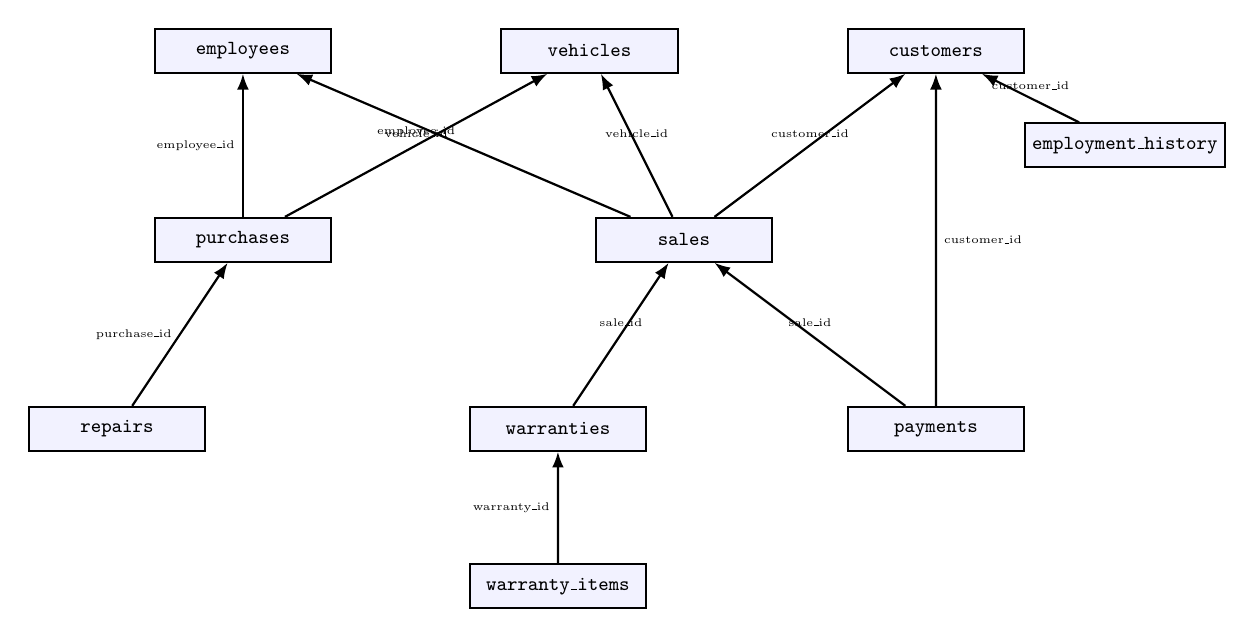
\begin{tikzpicture}[node distance=1.2cm, scale=0.8, every node/.style={scale=0.8}]

% Table boxes
\node[tablebox] (emp) at (0, 0) {employees};
\node[tablebox] (veh) at (5.5, 0) {vehicles};
\node[tablebox] (cust) at (11, 0) {customers};
\node[tablebox] (pur) at (0, -3) {purchases};
\node[tablebox] (sal) at (7, -3) {sales};
\node[tablebox] (eh) at (14, -1.5) {employment\_history};
\node[tablebox] (rep) at (-2, -6) {repairs};
\node[tablebox] (war) at (5, -6) {warranties};
\node[tablebox] (pay) at (11, -6) {payments};
\node[tablebox] (wi) at (5, -8.5) {warranty\_items};

% FK arrows (child -> parent)
\draw[-{Latex[length=2mm]}, thick] (pur) -- node[left, font=\tiny] {employee\_id} (emp);
\draw[-{Latex[length=2mm]}, thick] (pur) -- node[above, font=\tiny] {vehicle\_id} (veh);
\draw[-{Latex[length=2mm]}, thick] (rep) -- node[left, font=\tiny] {purchase\_id} (pur);
\draw[-{Latex[length=2mm]}, thick] (sal) -- node[above left, font=\tiny] {employee\_id} (emp);
\draw[-{Latex[length=2mm]}, thick] (sal) -- node[above, font=\tiny] {vehicle\_id} (veh);
\draw[-{Latex[length=2mm]}, thick] (sal) -- node[above, font=\tiny] {customer\_id} (cust);
\draw[-{Latex[length=2mm]}, thick] (eh) -- node[above, font=\tiny] {customer\_id} (cust);
\draw[-{Latex[length=2mm]}, thick] (war) -- node[above, font=\tiny] {sale\_id} (sal);
\draw[-{Latex[length=2mm]}, thick] (pay) -- node[above, font=\tiny] {sale\_id} (sal);
\draw[-{Latex[length=2mm]}, thick] (pay) -- node[right, font=\tiny] {customer\_id} (cust);
\draw[-{Latex[length=2mm]}, thick] (wi) -- node[left, font=\tiny] {warranty\_id} (war);

\end{tikzpicture}
\caption{Relational Schema with Foreign Key Relationships}
\label{fig:schema}
\end{figure}

\subsection{Normalization}

The prof covered normalization in Weeks 12 and 13, going through 1NF, 2NF, 3NF, and BCNF. All of my tables are in 3NF. There are no partial dependencies since every primary key is a single-column AUTO\_INCREMENT integer, which means 2NF is satisfied automatically. There are no transitive dependencies either: each non-key attribute depends directly on the primary key of its table, not on some other non-key column.

That said, I did make two deliberate denormalizations. The first is \texttt{num\_late\_payments} and \texttt{avg\_days\_late} on the customers table. Technically I could calculate these from the payments table every time, but the payment form spec required showing them. Recalculating with an aggregate query on every page load seemed slow and unnecessary, so I stored them directly on the customer record. It is a trade-off between strict normalization and performance.

The second is \texttt{customer\_id} on the payments table. That info already exists on the sales table (which payments link to through \texttt{sale\_id}), so it is redundant. But having it directly on payments means I do not need to JOIN through sales every time I want to look up a customer's payment history. It is another deliberate choice for query simplicity.

The prof talked about how BCNF is stricter than 3NF, but for this project 3NF was the right target. The two denormalizations are documented and intentional.

%==============================================================
\section{Stage 3: Forms and Reports}

Stage 3 was where the bulk of the coding happened. I built 6 input forms and 6 output reports, all in PHP with mysqli for the database calls. The forms follow the two-file pattern from the class tutorials: an HTML form collects the input, and a PHP processor script handles the INSERT.

\subsection{Input Forms}

\subsubsection*{Purchase Form (\texttt{purchase\_form.php})}

This form records a car bought at auction. The top section captures purchase info: date, location, seller/dealer name, and a checkbox for whether it was an auction purchase. The buyer employee gets selected from a dropdown populated from the employees table, filtered to only show people with the buyer role. The middle section is the vehicle details: make, model, year, color, miles, condition (dropdown with Excellent/Good/Fair/Poor), book price, style (Sedan/SUV/Truck/Van/Coupe), interior color, and price paid. The bottom section has up to 5 repair rows where you enter a problem description, estimated cost, and actual cost. Submitting the form inserts into three tables: vehicles, purchases, and repairs.

\textit{[Screenshot: Purchase Form]}

\subsubsection*{Sale Form (\texttt{sale\_form.php})}

This one records a car sale. There is a toggle at the top for choosing between an existing customer and a new one. If you pick ``New Customer,'' a set of fields appears for entering their info: name, phone, address, city, state, zip, gender, and date of birth. If you pick ``Existing Customer,'' you just select from a dropdown. The vehicle is selected from a list of available cars. Then there are the sale details: date, sale price, total due, down payment, financed amount, and commission. At the bottom there is space for up to 3 employment history entries for the customer. The tricky part was the existing/new customer toggle since it changes which fields show up on the page. Submitting inserts into sales and employment\_history, creates a new customer record if needed, and updates the vehicle status to sold.

\textit{[Screenshot: Sale Form]}

\subsubsection*{Warranty Form (\texttt{warranty\_form.php})}

This form adds warranty coverage to an existing sale. You pick a sale from a dropdown that shows the customer name, vehicle info, and sale date. When you select a sale, it fills in the vehicle, customer, and employee IDs using hidden fields and a bit of JavaScript. Then you enter the overall warranty details: date, total cost, and monthly cost. Below that there are up to 3 warranty item rows, each with a type dropdown (Drive-Train, Exterior, Interior, Electrical), start date, length in months, cost, deductible, and a text area for items covered. Submitting inserts into the warranties and warranty\_items tables.

\textit{[Screenshot: Warranty Form]}

\subsubsection*{Payment Form (\texttt{payment\_form.php})}

This form records a customer payment. There is a customer dropdown at the top that reloads the page when you select someone, so it can show that customer's info and existing payments below. Once a customer is selected, you see their gender, date of birth, number of late payments, and average days late. Then you pick which sale the payment is for, and enter the payment date, due date, paid date, amount, and bank account. If the paid date is after the due date, it gets flagged as late and the customer's late payment stats get recalculated. Below the form there is a table showing all existing payments for that customer, with late ones highlighted in red.

\textit{[Screenshot: Payment Form]}

\subsubsection*{Customer Form (\texttt{customer\_form.php})}

This is a simple add-and-view form. The top half has input fields for first name, last name, phone, address, city, state/province (defaults to AB), zip/postal code, gender, and date of birth. When you submit, it inserts into the customers table. Below the form there is a table showing all existing customers with their contact info, late payment count, and average days late.

\textit{[Screenshot: Customer Form]}

\subsubsection*{Employee Form (\texttt{employee\_form.php})}

Same pattern as the customer form. The input section has fields for first name, last name, phone, and a role dropdown (salesperson, buyer, or both). Existing employees are shown in a table below with their ID, name, phone, and role. Inserts into the employees table on submit.

\textit{[Screenshot: Employee Form]}

\subsection{Output Reports}

The reports are read-only pages that pull data from the database and display it in HTML tables. Most of them have some kind of filter so you can narrow down what you are looking at.

\subsubsection*{Current Inventory (\texttt{inventory.php})}

Shows all vehicles with status ``available.'' There is a text input at the top for filtering by make. For each car it shows make, model, year, color, miles, condition, book price, price paid, and total repair costs summed from the repairs table. It also calculates a total cost column (price paid plus repairs). The query uses a JOIN between vehicles and purchases, plus a subquery on repairs.

\textit{[Screenshot: Current Inventory Report]}

\subsubsection*{Sales Summary (\texttt{sales\_report.php})}

Shows all completed sales. You can filter by date range using a from/to date picker. For each sale it shows the date, vehicle info, customer name, salesperson, sale price, purchase cost, repair costs, and profit. The profit calculation was one of the trickier queries since it pulls from vehicles, purchases, repairs, sales, customers, and employees. Profit numbers are color-coded green for positive and red for negative. There is a totals row at the bottom.

\textit{[Screenshot: Sales Summary Report]}

\subsubsection*{Payment History (\texttt{payment\_history.php})}

You select a customer from a dropdown, and it shows all their payments in a table. The dropdown auto-submits when you change the selection. Each row shows the vehicle, due date, paid date, amount, bank account, days late, and status. Late payments (where \texttt{paid\_date} is after \texttt{due\_date}) get a red highlight using a CSS class. The query JOINs payments, sales, and vehicles.

\textit{[Screenshot: Payment History Report]}

\subsubsection*{Repair Costs (\texttt{repair\_summary.php})}

Shows estimated vs actual repair costs for every repair in the system. Each row has the vehicle info, purchase date, problem number, description, estimated cost, actual cost, and the difference. Rows where the actual cost exceeded the estimate get highlighted. This helps the dealership see which purchases ended up costing more to fix than they expected.

\textit{[Screenshot: Repair Costs Report]}

\subsubsection*{Active Warranties (\texttt{warranty\_report.php})}

Lists all warranty items with their expiry info. The page color-codes rows by urgency: red background for expired warranties, yellow background for ones expiring within 30 days, and no color for ones with more time left. Each row shows customer name, vehicle, warranty type, start date, length in months, expiry date, days remaining, cost, deductible, and items covered. The query JOINs warranties, warranty\_items, vehicles, and customers.

\textit{[Screenshot: Active Warranties Report]}

\subsubsection*{Late Payments (\texttt{late\_payments.php})}

Shows all customers who have at least one late payment, sorted worst-first by late count. Each row has the customer name, phone, total payments, number of late payments, and average days late. It uses a GROUP BY on customer with a HAVING clause to only show customers where \texttt{late\_count} is greater than zero. This is basically a credit risk report for the dealership.

\textit{[Screenshot: Late Payments Report]}

%==============================================================
\section{Stage 4: Business Queries}

The project spec required at least 10 queries with at least 5 being advanced (multi-table JOINs or subqueries). I ended up with 12 total: 5 simple and 7 advanced. They are all on a single queries page with a dropdown selector. You pick a query, hit submit, and the results show up in a table below.

For Query 3 there is also a text input so you can search by make. The SQL for each query is shown on the page along with the results, which is helpful for debugging and for the demo.

%--------------------------------------------------------------
\subsection{Query 1: What cars do we have on the lot right now? (Simple)}

This one pulls up every vehicle that is still available for sale. It is the quickest way for a salesperson to see what is on the lot without walking outside.

\begin{lstlisting}[style=sql]
SELECT * FROM vehicles
WHERE status = 'available'
ORDER BY make, model
\end{lstlisting}

\textbf{SQL features:} basic SELECT with WHERE, ORDER BY

%--------------------------------------------------------------
\subsection{Query 2: Show me all our customers (Simple)}

Lists every customer in the system with their contact info. Useful for the office staff when they need to look someone up or check a phone number.

\begin{lstlisting}[style=sql]
SELECT customer_id, first_name, last_name, phone, city, state
FROM customers
ORDER BY last_name
\end{lstlisting}

\textbf{SQL features:} basic SELECT with ORDER BY

%--------------------------------------------------------------
\subsection{Query 3: Do we have any [make] cars in stock? (Simple)}

This one takes a text input for the make, so the actual query uses the value the user types in. It is for when a customer calls and asks ``do you have any Toyotas?'' and you need a quick answer.

\begin{lstlisting}[style=sql]
SELECT * FROM vehicles
WHERE make = '[make]' AND status = 'available'
\end{lstlisting}

\textbf{SQL features:} WHERE with parameter, AND condition

%--------------------------------------------------------------
\subsection{Query 4: Who are our employees? (Simple)}

Shows all employees sorted by their role and last name. Pretty straightforward, just a quick reference for who works here and what they do.

\begin{lstlisting}[style=sql]
SELECT * FROM employees
ORDER BY role, last_name
\end{lstlisting}

\textbf{SQL features:} basic SELECT with ORDER BY

%--------------------------------------------------------------
\subsection{Query 5: How many cars did we buy this month? (Simple)}

Gives a count of purchases made in the current month along with the total amount spent. The MONTH() and YEAR() functions with CURDATE() make it automatically filter to the current month.

\begin{lstlisting}[style=sql]
SELECT COUNT(*) as cars_bought, SUM(price_paid) as total_spent
FROM purchases
WHERE MONTH(purchase_date) = MONTH(CURDATE())
AND YEAR(purchase_date) = YEAR(CURDATE())
\end{lstlisting}

\textbf{SQL features:} COUNT, SUM aggregates, MONTH/YEAR functions with CURDATE()

%--------------------------------------------------------------
\subsection{Query 6: Which cars did we buy below book price? (Advanced)}

This one is useful for the buyers to see which deals paid off. It joins vehicles and purchases to compare what was paid against the book price, then calculates the savings.

\begin{lstlisting}[style=sql]
SELECT v.make, v.model, v.year, v.book_price, p.price_paid,
       (v.book_price - p.price_paid) as savings
FROM vehicles v
JOIN purchases p ON v.vehicle_id = p.vehicle_id
WHERE p.price_paid < v.book_price
ORDER BY savings DESC
\end{lstlisting}

\textbf{SQL features:} JOIN between vehicles and purchases, calculated column (savings)

%--------------------------------------------------------------
\subsection{Query 7: What is our profit on each sale? (Advanced)}

This was the hardest query to write. The profit calculation needs to factor in the purchase price AND all repair costs, so there is a correlated subquery that sums repairs for each purchase. The COALESCE handles cases where a vehicle had no repairs so the sum does not come back as NULL.

\begin{lstlisting}[style=sql]
SELECT v.make, v.model, v.year, s.sale_price, p.price_paid,
       (SELECT COALESCE(SUM(r.actual_cost),0) FROM repairs r
        WHERE r.purchase_id = p.purchase_id) as repair_costs,
       (s.sale_price - p.price_paid -
        (SELECT COALESCE(SUM(r.actual_cost),0) FROM repairs r
         WHERE r.purchase_id = p.purchase_id)) as profit
FROM sales s
JOIN vehicles v ON s.vehicle_id = v.vehicle_id
JOIN purchases p ON v.vehicle_id = p.vehicle_id
ORDER BY profit DESC
\end{lstlisting}

\textbf{SQL features:} correlated subquery for repair costs, multiple JOINs (sales + vehicles + purchases), COALESCE, calculated profit

%--------------------------------------------------------------
\subsection{Query 8: Which customers have late payments? (Advanced)}

Shows every late payment along with the customer name, vehicle info, and how many days late it was. The DATEDIFF function calculates how many days late each payment was. The prof covered date functions in the Week 6 lectures.

\begin{lstlisting}[style=sql]
SELECT DISTINCT CONCAT(c.first_name, ' ', c.last_name) as customer_name,
       c.phone, v.make, v.model, v.year,
       DATEDIFF(pay.paid_date, pay.due_date) as days_late
FROM payments pay
JOIN customers c ON pay.customer_id = c.customer_id
JOIN sales s ON pay.sale_id = s.sale_id
JOIN vehicles v ON s.vehicle_id = v.vehicle_id
WHERE pay.paid_date > pay.due_date
ORDER BY days_late DESC
\end{lstlisting}

\textbf{SQL features:} 4-table JOIN (payments + customers + sales + vehicles), DATEDIFF, DISTINCT, WHERE on date comparison

%--------------------------------------------------------------
\subsection{Query 9: Who is our top salesperson? (Advanced)}

Groups sales by employee and shows their total revenue and commission. The COUNT gives number of sales and SUM gives the dollar totals. Sorted by number of sales so the top performer shows up first.

\begin{lstlisting}[style=sql]
SELECT CONCAT(e.first_name, ' ', e.last_name) as salesperson,
       COUNT(s.sale_id) as num_sales,
       SUM(s.sale_price) as total_revenue,
       SUM(s.commission) as total_commission
FROM sales s
JOIN employees e ON s.employee_id = e.employee_id
GROUP BY e.employee_id
ORDER BY num_sales DESC
\end{lstlisting}

\textbf{SQL features:} JOIN, GROUP BY, COUNT, SUM aggregates

%--------------------------------------------------------------
\subsection{Query 10: Which warranties expire within 90 days? (Advanced)}

This uses DATE\_ADD to calculate the expiry date from start\_date + length\_months, then BETWEEN to check if it falls within the next 90 days. The DATEDIFF gives the exact number of days remaining so the dealership can follow up with customers before their coverage runs out.

\begin{lstlisting}[style=sql]
SELECT CONCAT(c.first_name, ' ', c.last_name) as customer_name,
       v.make, v.model, v.year,
       wi.warranty_type, wi.start_date,
       DATE_ADD(wi.start_date, INTERVAL wi.length_months MONTH)
           as expiry_date,
       DATEDIFF(DATE_ADD(wi.start_date,
           INTERVAL wi.length_months MONTH), CURDATE())
           as days_remaining
FROM warranty_items wi
JOIN warranties w ON wi.warranty_id = w.warranty_id
JOIN vehicles v ON w.vehicle_id = v.vehicle_id
JOIN customers c ON w.customer_id = c.customer_id
WHERE DATE_ADD(wi.start_date, INTERVAL wi.length_months MONTH)
      BETWEEN CURDATE() AND DATE_ADD(CURDATE(), INTERVAL 90 DAY)
ORDER BY expiry_date
\end{lstlisting}

\textbf{SQL features:} DATE\_ADD, DATEDIFF, BETWEEN with date range, 4-table JOIN

%--------------------------------------------------------------
\subsection{Query 11: Where did repair costs go over budget? (Advanced)}

The HAVING clause filters groups to only show vehicles where actual repair costs exceeded estimates. The prof covered the difference between WHERE and HAVING in Week 6: WHERE filters individual rows before grouping, HAVING filters groups after. This query groups repairs by purchase and compares the totals.

\begin{lstlisting}[style=sql]
SELECT v.make, v.model, v.year,
       SUM(r.est_cost) as estimated_total,
       SUM(r.actual_cost) as actual_total,
       (SUM(r.actual_cost) - SUM(r.est_cost)) as over_budget
FROM repairs r
JOIN purchases p ON r.purchase_id = p.purchase_id
JOIN vehicles v ON p.vehicle_id = v.vehicle_id
GROUP BY p.purchase_id
HAVING SUM(r.actual_cost) > SUM(r.est_cost)
ORDER BY over_budget DESC
\end{lstlisting}

\textbf{SQL features:} GROUP BY with HAVING, SUM aggregates, calculated column

%--------------------------------------------------------------
\subsection{Query 12: Which customers bought more than one car? (Advanced)}

Simple but useful. \texttt{HAVING COUNT(s.sale\_id) > 1} keeps only repeat buyers. This is good for identifying loyal customers who might be interested in future deals.

\begin{lstlisting}[style=sql]
SELECT CONCAT(c.first_name, ' ', c.last_name) as customer_name,
       c.phone,
       COUNT(s.sale_id) as cars_bought,
       SUM(s.sale_price) as total_spent
FROM customers c
JOIN sales s ON c.customer_id = s.customer_id
GROUP BY c.customer_id
HAVING COUNT(s.sale_id) > 1
ORDER BY cars_bought DESC
\end{lstlisting}

\textbf{SQL features:} GROUP BY with HAVING COUNT, aggregate functions

%==============================================================
\section{Assumptions and Design Decisions}

Here are the main assumptions I made and the reasoning behind the bigger design decisions.

\begin{enumerate}
  \item \textbf{Used \texttt{condition\_desc} instead of \texttt{condition}}: MySQL has \texttt{condition} as a reserved word, so I could not use it as a column name without backticks everywhere. Renaming to \texttt{condition\_desc} was the simplest fix. Not ideal but clear enough.

  \item \textbf{Denormalized late payment stats on customers table}: The \texttt{num\_late\_payments} and \texttt{avg\_days\_late} columns on the customers table are technically redundant since they could be calculated from the payments table each time. But the payment form spec required showing these values, and recalculating on every page load with an aggregate query would be slower. I chose to store them directly and update them whenever a late payment is recorded. The prof talked about how normalization trades some redundancy for query performance; this is one of those trade-offs.

  \item \textbf{\texttt{customer\_id} duplicated on payments}: The payments table has \texttt{customer\_id} even though you could get it by joining through sales. It is there so I can quickly look up all payments for a customer without an extra JOIN. Another deliberate denormalization.

  \item \textbf{AUTO\_INCREMENT surrogate keys everywhere}: Every table uses an INT AUTO\_INCREMENT primary key instead of composite or natural keys. It is simpler for foreign key references and avoids issues if natural values change. The prof covered candidate keys and primary key selection in Week 2; I went with surrogate keys because they are straightforward.

  \item \textbf{Tables created in FK dependency order}: The \texttt{db\_setup.sql} file creates tables in the right order (employees and vehicles first, then purchases, etc.) so the foreign key constraints do not fail. This way the script runs straight through without needing deferred constraint checks.

  \item \textbf{Alberta-specific sample data}: All the seed data uses Lethbridge, Calgary, and Medicine Hat locations with Alberta postal codes. Keeps it realistic for the course context.

  \item \textbf{Deliberate late payment data in seed}: I included some payment records where \texttt{paid\_date} is after \texttt{due\_date} on purpose, so the late payment reports and queries actually have data to show during testing and the demo.
\end{enumerate}

%==============================================================
\section{What I Learned}

The biggest thing I took away from this project is how normalization actually works in practice. In lectures, the prof walked through functional dependencies and decomposition on paper (Weeks 12--13), but actually deciding where to denormalize for a real application was a different kind of challenge. It is one thing to identify a transitive dependency; it is another to decide whether the performance trade-off is worth it.

I had never used PHP before this course. The procedural mysqli pattern from the tutorials turned out to be pretty straightforward once I got the hang of it. The hardest part was debugging SQL errors since PHP just gives you a generic error string and you have to figure out which part of the query is wrong.

Drawing the E-R diagram first and then mapping it to relational tables (Week 11 material) made the schema design way more structured than if I had just started creating tables. It forced me to think about relationships and cardinalities before writing any SQL.

Setting up the foreign keys caught several data integrity issues during testing. I tried inserting a sale for a \texttt{vehicle\_id} that did not exist and MySQL blocked it. That is exactly what referential integrity is supposed to do, and it is way better than having orphaned records.

Writing the advanced queries (especially Query 7 with the correlated subquery) pushed me to actually understand how JOINs and subqueries work together. The prof's examples in Weeks 6 and 8 used the banking database, but applying those patterns to a different domain helped it click.

%==============================================================
\section{Future Improvements}

If I had more time or was building this for a real dealership, here is what I would add:

\begin{enumerate}
  \item \textbf{User login system}: Right now anyone can access everything. A real system would need separate logins for buyers, salespeople, and managers, with different permissions for each. The prof mentioned security as one of the topics related to DB systems in Week 1.

  \item \textbf{Search and sorting on reports}: The reports have basic filters but you cannot sort by clicking column headers or search within results. Adding JavaScript for client-side sorting would make the reports much more usable.

  \item \textbf{Mobile/responsive layout}: The forms use HTML tables for layout, which does not work great on phones. The buyers at auctions mentioned wanting a portable version, so a responsive design would be a big improvement.

  \item \textbf{Credit bureau integration}: The spec mentions that really bad customers get reported to the credit bureau. Right now there is no integration for that. An API connection to a credit reporting service would automate that process.

  \item \textbf{Inventory alerts}: The dealership tries to keep no more than 50 cars on the lot. An alert system that warns when inventory is getting high (or when popular makes are running low) would help the buyers make better decisions at auctions.
\end{enumerate}

Overall I am pretty happy with how the project turned out. It covers the full lifecycle from buying cars to collecting payments, and the queries answer real business questions that a dealership would actually care about.

\end{document}
